% !TEX TS-program = pdfLaTeX+MakeIndex+BibTeX
% !TEX encoding = UTF-8 Unicode

\PassOptionsToPackage{unicode}{hyperref}
\PassOptionsToPackage{naturalnames}{hyperref}

\documentclass[tg]{mdtufsm}

\usepackage[T1]{fontenc}
\usepackage{fix-cm}
\usepackage{times, color}
\usepackage[utf8]{inputenc}
\usepackage{graphicx}
\usepackage{amsmath,latexsym,amssymb}
%\usepackage[hidelinks]{hyperref}
\usepackage[hidelinks,
            bookmarksopen=true,linktoc=none,colorlinks=true,
            linkcolor=black,citecolor=black,filecolor=magenta,urlcolor=blue,
            pdftitle={Exploração da Linguagem Rust para o Desenvolvimento de um Path Tracer Paralelo},
            pdfauthor={Yuri Kunde Schlesner},
            pdfsubject={Trabalho de Graduação},
            pdfkeywords={Computação Gráfica, Linguagens de Programação, Programação Paralela, Rust, Path Tracing, Informática, UFSM}
            ]{hyperref}
%\usepackage[brazilian]{babel}

%\usepackage{fontspec}
%\setmainfont{Linux Libertine G}

%%% PAGE DIMENSIONS
\usepackage[inner=30mm,outer=20mm,top=30mm,bottom=20mm]{geometry} 
\usepackage{epstopdf}
\usepackage{graphicx}
% \geometry{margin=2in} % for example, change the margins to 2 inches all round
% \geometry{landscape} % set up the page for landscape

% \usepackage[parfill]{parskip} % Activate to begin paragraphs with an empty line rather than an indent

%%% PACKAGES
%\usepackage{amsfonts}
%\usepackage{color}
%\usepackage{booktabs} % for much better looking tables
%\usepackage{array} % for better arrays (eg matrices) in maths
%\usepackage{paralist} % very flexible & customisable lists (eg. enumerate/itemize, etc.)
\usepackage{verbatim} % adds environment for commenting out blocks of text & for better verbatim
\usepackage{listings}
\usepackage{parcolumns}
%\usepackage{microtype}
%\usepackage[numbers]{natbib}
%\usepackage{subfig} % make it possible to include more than one captioned figure/table in a single float
% These packages are all incorporated in the memoir class to one degree or another...

\lstset{
	basicstyle=\scriptsize\ttfamily,
	tabsize=2,
	frame=single,
	breaklines=true,
	breakatwhitespace=true,
	xleftmargin=0cm,
	xrightmargin=0cm,
	literate=
		{á}{{\'a}}1 {é}{{\'e}}1 {í}{{\'i}}1 {ó}{{\'o}}1 {ú}{{\'u}}1
		{Á}{{\'A}}1 {É}{{\'E}}1 {Í}{{\'I}}1 {Ó}{{\'O}}1 {Ú}{{\'U}}1
		{à}{{\`a}}1 {è}{{\`e}}1 {ì}{{\`i}}1 {ò}{{\`o}}1 {ù}{{\`u}}1
		{À}{{\`A}}1 {È}{{\'E}}1 {Ì}{{\`I}}1 {Ò}{{\`O}}1 {Ù}{{\`U}}1
		{ä}{{\"a}}1 {ë}{{\"e}}1 {ï}{{\"i}}1 {ö}{{\"o}}1 {ü}{{\"u}}1
		{Ä}{{\"A}}1 {Ë}{{\"E}}1 {Ï}{{\"I}}1 {Ö}{{\"O}}1 {Ü}{{\"U}}1
		{â}{{\^a}}1 {ê}{{\^e}}1 {î}{{\^i}}1 {ô}{{\^o}}1 {û}{{\^u}}1
		{Â}{{\^A}}1 {Ê}{{\^E}}1 {Î}{{\^I}}1 {Ô}{{\^O}}1 {Û}{{\^U}}1
		{ã}{{\~a}}1 {Ã}{{\~A}}1
		{ç}{{\c c}}1 {Ç}{{\c C}}1
}

% For Computer Modern:
%\def\Cpp{{C\nolinebreak[4]\hspace{-.05em}\raisebox{.4ex}{\tiny\bf ++}}}
% For Linux Libertine G
\def\Cpp{{C\nolinebreak[4]\raisebox{.20ex}{\small\bf++}}}

\newcommand{\todo}[1]{\textsf{\color{red}#1}}


%%=============================================================================
%% Trampa para corrigir o bug do hyperref que redefine o caption das figuras e das
%% tabelas, n�o colocando o nome ``Figura'' antes do n�mero do mesmo na lista
%%=============================================================================

\makeatletter

\long\def\@caption#1[#2]#3{%
  \expandafter\ifx\csname if@capstart\expandafter\endcsname
                  \csname iftrue\endcsname
    \global\let\@currentHref\hc@currentHref
  \else
    \hyper@makecurrent{\@captype}%
  \fi
  \@ifundefined{NR@gettitle}{%
    \def\@currentlabelname{#2}%
  }{%
    \NR@gettitle{#2}%
  }%
  \par\addcontentsline{\csname ext@#1\endcsname}{#1}{%
    \protect\numberline{\csname fnum@#1\endcsname ~-- }{\ignorespaces #2}%
  }%
  \begingroup
    \@parboxrestore
    \if@minipage
      \@setminipage
    \fi
    \normalsize
    \expandafter\ifx\csname if@capstart\expandafter\endcsname
                    \csname iftrue\endcsname
      \global\@capstartfalse
      \@makecaption{\csname fnum@#1\endcsname}{\ignorespaces#3}%
    \else
      \@makecaption{\csname fnum@#1\endcsname}{%
        \ignorespaces
        \ifHy@nesting
          \expandafter\hyper@@anchor\expandafter{\@currentHref}{#3}%
        \else
          \Hy@raisedlink{%
            \expandafter\hyper@@anchor\expandafter{%
              \@currentHref
            }{\relax}%
          }%
          #3%
        \fi
      }%
    \fi
    \par
  \endgroup
}

\makeatother

%%% END Article customizations

\title{Exploração da Linguagem Rust para o Desenvolvimento de um \emph{Path Tracer} Paralelo}
\author{Schlesner}{Yuri Kunde}
\course{Curso de Ciência da Computação}
\altcourse{Curso de Ciência da Computação}
\institute{Centro de Tecnologia}
\degree{Bacharel em Ciência da Computação}

\trabalhoNumero{}
\advisor[Profª.]{Drª.}{Charão}{Andrea Schwertner}
\orientadoratrue

\committee[Profª. Drª.]{Augustin}{Iara}{UFSM}
\committee[Prof. Dr.]{Lima}{João Vicente Ferreira}{UFSM}

\date{20}{Outubro}{2014}

\keyword{Computação Gráfica}
\keyword{Linguagens de Programação}
\keyword{Programação Paralela}
\keyword{Rust}
\keyword{Path Tracing}

%\date{} % Activate to display a given date or no date (if empty), otherwise the current date is printed

\begin{document}
\maketitle
\makeapprove

\begin{abstract}
A Computação Gráfica, e especificamente a geração de imagens por computador, é uma área com
inúmeras aplicações. No entanto, para a geração de imagens realísticas, é essencial fazer
uso eficiente do poder computacional disponível, pois é um processo quer requer a realização
de um grande número de cálculos. Tradicionalmente foram utilizadas linguagens como \Cpp, que
permitem esta eficiência, para escrever estes tipos de sistemas. \emph{Rust}, uma nova
linguagem de sistemas, tem como um dos seus objetivos servir este nicho de aplicação. Este
trabalho tem como objetivo re-implementar um renderizador fotorrealista utilizando Rust,
afim de avaliar se a linguagem realmente atende as necessidades deste tipo de aplicação.
\end{abstract}

\tableofcontents

\setlength{\baselineskip}{1.5\baselineskip}

%	\item[Período de execução:] Setembro de 2014 a Dezembro de 2014
%	\item[Unidades participantes:] ~\\ Curso de Ciência da Computação \\ Departamento de Eletrônica e Computação
%	\item[Área de conhecimento:] Ciência da Computação
%	\item[Linha de Pesquisa:] Computação Gráfica, Linguagens de Programação, Programação Paralela
%	\item[Tipo de projeto:] Trabalho de Conclusão de Curso

\chapter{Introdução}

A \emph{Computação Gráfica} é a área da Ciência da Computação que estuda tópicos relacionados à
criação, análise e manipulação de imagens e conceitos relacionados. Dentre estas, a síntese (ou
renderização) de imagens é onde uma imagem é criada de forma computacional, a partir de um modelo
matemático e frequentemente buscando o fotorrealismo. Tem uma vasta quantidade de aplicações
práticas: É usada na engenharia, durante o projeto de máquinas ou construções; na arquitetura, para
a visualização de espaços; para entretenimento, em efeitos especiais de filmes ou em jogos 3D e
muitas outras.

Como a geração de imagens fotorrealistas envolve essencialmente uma simulação completa da física da
luz, um processo proibitivamente lento e complexo, são utilizadas simplificações e modelos. No
passado, devido a limitada capacidade computacional disponível, eram utilizadas aproximações
grosseiras que, embora produzissem imagens atrativas, não eram muito realísticas, especialmente no
quesito da aparência das superfícies e de suas interações com a luz. Com o aumento do poder
computacional disponível, vem sendo usados modelos mais fiéis à realidade e que produzem imagens
mais convincentes, algumas vezes indistinguíveis de uma fotografia real.

\emph{Path tracing} é um método de renderização que assume que a luz se comporta como uma partícula
e calcula uma imagem traçando uma série de raios pelos caminhos através quais a luz viajaria quando
refletida através de uma cena. Atualmente é um dos algoritmos mais usados quando são demandadas
imagens com um grau de realismo extremamente alto, devido a sua habilidade de simular o
comportamento da luz com relativa precisão.

No entanto, este realismo vem ao custo de muito poder de processamento, e mesmo com o avanço
tecnológico de CPUs, a renderização de imagens continua sendo uma tarefa árdua para processadores.
Sistemas de renderização profissionais são quase exclusivamente escritos em \Cpp\ e não em
linguagens de mais alto nível, devido as penalidades de performance que impõem. Sistemas mais
recentes chegam a fazer o uso de GPUs para acelerar a imensa quantidade de cálculos necessária.
Tendo em vista a baixa expressividade de \Cpp\ comparada a estas outras linguagens, torna-se
interessante explorar alternativas que permitam mais fácil desenvolvimento mas sem sacrificar a
performance requerida.

A linguagem de programação \emph{Rust}, um projeto de pesquisa da \emph{Mozilla Research}, tem como
seu objetivo ser uma união entre linguagens de programação de sistemas e as tidas como ``linguagens
de alto-nível'', focando simultaneamente em alta-performance, segurança e expressividade. Ela atinge
isso usando um modelo tradicional de compilação prévia (\emph{ahead of time}) e um sistema de tipos
que permite a verificação automática dos usos de ponteiros durante a compilação, eliminando a
possibilidade de acontecerem erros de memória sem introduzir penalidades excessivas de performance
ou consumo de memória. Ao mesmo tempo, integra conceitos mais recentes de linguagens de programação
que aumentam sua expressividade e capacidade de facilmente descrever programas complexos.

\section{Objetivos}

\subsection{Objetivo Geral}

O objetivo geral deste trabalho é portar um \emph{path tracer} para \emph{Rust} e, através deste processo,
realizar uma comparação qualitativa e quantitativa entre esta linguagem e \Cpp, nos aspectos de
performance e organização de código. Como base será utilizado o SmallVCM\citep{smallvcm}, um
\emph{path tracer} de propósito educativo escrito em \Cpp, escolhido por implementar uma variedade
de algoritmos diferentes de \emph{path tracing} e por ser relativamente compacto, consistindo de
aproximadamente 5000 linhas de código.

\subsection{Objetivos Específicos}
\begin{itemize}
	\item Estudar o código original do SmallVCM.
	\item Re-escrever um subconjunto mínimo do SmallVCM utilizando Rust, para a realização de
		testes.
	\item Realizar uma comparação de performance e clareza de código entre as duas versões e
		identificar possíveis melhorias.
	\item Paralelizar o renderizador, afim de melhorar sua performance, fazendo uso das
		funcionalidades de Rust.
	\item Portar o restante do SmallVCM, afim de que as duas versões tenham funcionalidades
		equivalentes.
\end{itemize}

\section{Justificativa}

Rust é uma linguagem relativamente nova e, embora aplicações gráficas de alta performance sejam um
dos seus públicos alvo, ainda não existe uma quantidade significativa de programas deste tipo que
valide a linguagem para este propósito. A experiência e resultados adquiridos durante a realização
deste trabalho podem ajudar a guiar o desenvolvimento da linguagem para atingir este fim.

\chapter{Fundamentos e Revisão de Literatura}

Neste capítulo será dada uma descrição dos conceitos teóricos das áreas de linguagens de programação e de computação gráfica nas quais o trabalho e as ferramentas nele utilizadas, a linguagem de programação \emph{Rust} e o algoritmo de \emph{path tracing}, se baseiam.

\section{Rust}

Rust\citep{rust} é uma linguagem de programação de propósito geral, oficialmente patrocinada pela
\emph{Mozilla Research} mas desenvolvida também pela comunidade. É uma linguagem de propósito geral,
que busca atender as necessidades de programadores que atualmente utilizariam linguagens como C ou
\Cpp, por questões de performance ou de controle sobre o hardware. Uma de suas características mais
distintivas é o modelo de referências que utiliza, baseado em regiões\citep{tofte1997}, que
automaticamente gerencia a vida de alocações de memória, evitando com que sejam feitos erros neste
gerenciamento, ou que memória inválida seja acessada pelo programa, sem necessitar o uso de um
\emph{garbage collector}. A linguagem foi originalmente desenvolvida para servir como linguagem de
implementação do projeto Servo\citep{servo}, um browser experimental de próxima geração também
desenvolvido pela Mozilla Research, mas atualmente já cresceu além deste objetivo para se tornar um
projeto maior.

Além de melhorias no gerenciamento de memória, a linguagem busca também trazer funcionalidades
tradicionalmente oferecidas em linguagens funcionais, trazendo uma forte inspiração de linguagens
como ML\citep{milner1997}. Assim, possui funcionalidades como \emph{pattern matching}, tuplas,
\emph{sum types} (também conhecidos como \emph{Algebraic Data Types} (ADTs) ou \emph{uniões
discriminadas}.) A linguagem não implementa o modelo tradicional de programação orientada a objetos,
oferecendo em troca o conceito de \emph{traits} (similares ao conceito de \emph{type classes} em
Haskell ou de \emph{interfaces} em outras linguagens) que evita alguns problemas do modelo baseado
em herança de classes, como a falta de extensibilidade de tipos e o \emph{problema diamante} em
herança múltipla\citep{scharli2003}.

O compilador oficial da linguagem, o \emph{rustc}, é implementado na própria linguagem e utiliza a
infraestrutura do projeto LLVM\citep{lattner2004}, permitindo que usufrua das capacidades de
otimização e geração de código do projeto para alcançar uma variedade de plataformas. O compilador
também tem suporte ao carregamento de \emph{plugins} durante o processo de análise, o que expõe
poderosas capacidades de meta-programação aos usuários. Alguns exemplos de projetos que utilizam
estas capacidades são o RustGPU\citep{holk2013}, que permite a compilação de código Rust para
execução paralela em GPUs, e Zinc\citep{zinc}, um \emph{framework} para desenvolvimento de
aplicações embarcadas em microprocessadores.

\section{\emph{Path Tracing}}

\emph{Path tracing} faz parte de uma família de algoritmos comumente denominados algoritmos de
\emph{ray tracing}. Embora também utilizados na física e nas engenharias, no contexto deste trabalho
são algoritmos que tem como finalidade a produção de imagens que retratam cenas tridimensionais.

Todos os algoritmos desta família se baseiam na ideia fundamental de simular o comportamento da luz
traçando raios que saem da câmera virtual em direção a cena. Isto é o contrário do que ocorre na
vida real, onde a luz é emitida de uma fonte e viaja pelo espaço até chegar ao observador, mas não
afeta negativamente o resultado final e torna o algoritmo computacionalmente viável, pois assegura
que todo o raio traçado é um que eventualmente chegaria no observador. (A maioria da luz numa cena
não chega até o observador, que subtende um espaço relativamente pequeno nela.)\citep{pharr2010}

Os primeiros algoritmos deste tipo a serem usados simplesmente traçavam um raio por pixel da imagem,
encontrando a intersecção deste raio com a cena e calculando sua aparência de acordo com algum
modelo básico de iluminação. Desta forma, não eram reproduzidas sombras nem superfícies refletivas,
como espelhos ou objetos metálicos. Estes tipo de algoritmos vieram a ser chamado de algoritmos de
\emph{ray casting}.

\Citet{whitted1980} propôs um novo método que soluciona estes problemas. Além do primeiro raio
partindo da câmera, são também traçados raios que vão do ponto sendo iluminado até cada uma das
fontes luminosas, permitindo que cada luz só seja adicionada se não estiver obstruída por outro
objeto e assim permitindo a renderização de sombras. Em superfícies refletivas, outro raio é traçado
na direção do reflexo, o qual é utilizado para calcular a luminosidade naquela direção, da mesma
maneira que o raio inicial. Assim, este algoritmo implementa \emph{ray tracing recursivo}.

\Citet{cook1984} aprimoraram o algoritmo de \citeauthor{whitted1980} para que suporte uma variedade
de efeitos adicionais como superfícies foscas e translúcidas, sombras com penumbras realísticas,
profundidade de campo e borrão de movimento. Todos estes efeitos são realizados através do mesmo
método de tirar várias amostras em cada ponto da imagem, introduzindo uma variação nas direções ou
posições traçadas em cada amostra. Embora não tenha o embasamento matemático, esta é a mesma ideia
básica utilizada posteriormente em algoritmos que utilizam integração Monte Carlo.

\Citet{kajiya1986} introduz a \emph{equação de renderização}, que descreve a interação da luz com as
superfícies, modelando também a reflexão de luz em superfícies completamente foscas (ver
\autoref{fig:path_tracing}.) Esta serve como uma importante fundação teórica que é usada como base
para o cálculo da imagem ou para o desenvolvimento de aproximações. No mesmo artigo é introduzida a
técnica de \emph{path tracing}, que difere das anteriores desenvolvidas por \citeauthor{cook1984} e
\citeauthor{whitted1980} por observar que os raios mais impactantes na aparência final da imagem são
os de baixa profundidade, e assim traçando apenas um raio recursivo por amostra, evitando o
crescimento exponencial do número de raios traçados que ocorre com as outras técnicas.

Embora capaz de produzir imagens extremamente realísticas, \emph{path tracing} pode requerer uma
quantidade impraticável de amostras para renderizar satisfatoriamente certos tipos de cenas onde não
exista uma linha de visão direta entre as superfícies e as fontes de luz. Nestas cenas a maioria da
iluminação se dá através de caminhos indiretos ou através de superfícies refratantes que projetam
padrões de luz complicados em outras superfícies (conhecidos como \emph{caustics}.) Para contornar
estes problemas foram desenvolvidas inúmeras extensões ao algoritmo de \emph{path tracing}. Dentre
elas se destaca \emph{bidirectional path tracing}, introduzido por \citet{lafortune1993}. Este
algoritmo foi depois reformulado por \citeauthor{veach1997} em \citep{veach1997}, onde também
introduziu a técnica de \emph{multiple importance sampling} e o algoritmo \emph{Metropolis light
transport}.

\begin{figure}
	\centering
	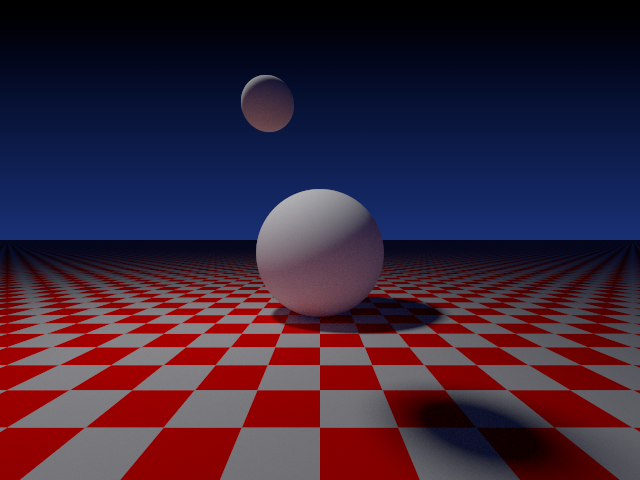
\includegraphics[width=0.5\textwidth]{exemplo_imagem}
	\caption{
		Um exemplo de uma imagem gerada utilizando \emph{path tracing}. Note como a luz que atinge o
		plano xadrez é refletida de volta para iluminar a esfera, um fenômeno conhecido como
		\emph{iluminação indireta} e que é corretamente simulado pelo algoritmo.
	}
	\label{fig:path_tracing}
\end{figure}

\chapter{Desenvolvimento}

Aqui serão descritas as atividades realizadas para atingir os objetivos propostos. Será dada uma explicação da organização do ambiente de compilação e desenvolvimento utilizadas nas versões do \emph{SmallVCM}. (A original e a re-escrita em \emph{Rust}, denominada \emph{SmallVCM-rs}.) Seguindo, será feita uma descrição da organização de código do \emph{SmallVCM}, e de como a implementação de seus componentes mudou no código \emph{Rust} por influência de diferenças entre essa linguagem e \Cpp.

\section{Ambiente de Desenvolvimento e Organização de Projeto}

\subsection{Rust}

O compilador \emph{rustc}, além de ser oficialmente distribuído em forma de código fonte, também é disponibilizado através de pacotes binários distribuídos na página do projeto\footnote{\url{http://www.rust-lang.org/install.html}}. Estes pacotes evitam que usuários passem pelo processo de \emph{bootstrap} do compilador, que pode levar de uma à varias horas, dependendo do hardware em que é executado. Atualizados diariamente, os pacotes binários são providos para os sistemas operacionais Linux, Mac OS X e Windows, em versões 32-bits ou 64-bits. Ocasionalmente são também feitas versões numeradas do compilador, porém seu uso não é recomendado pois rapidamente ficam defasadas, um problema se pretende-se utilizar qualquer biblioteca de terceiros.

Para o desenvolvimento, foi utilizada uma máquina virtual contendo o sistema operacional \emph{Arch Linux}. Além de conter software atualizado, existem pacotes de terceiros para a distribuição que automaticamente instalam versões atualizadas do compilador de Rust.\footnote{\url{https://aur.archlinux.org/packages/rust-nightly-bin/}} Como a linguagem ainda está em fase de mudança frequente, poder atualizar o compilador facilmente é importante para se manter atualizado com as últimas mudanças e funcionalidades incluídas diariamente na linguagem.

Além do compilador, também é utilizado o gerenciador de pacotes oficial \emph{Cargo}\footnote{\url{http://crates.io/}}, desenvolvido especificamente para gerenciar e compilar bibliotecas \emph{Rust}. Assim como o compilador, também existem pacotes \emph{Arch Linux} para manter este atualizado\footnote{\url{https://aur.archlinux.org/packages/cargo-nightly-bin/}}.

Seguindo sua estrutura recomendada de projeto, é possível utilizar o \emph{Cargo} para gerenciar a compilação, com o comando \texttt{cargo build}, evitando a necessidade de um \emph{Makefile}. Além das tarefas básicas de um build system, o sistema também encarrega-se de automaticamente fazer o download e instalação de quaisquer bibliotecas externas utilizadas. Neste trabalho, no entanto, esta funcionalidade não é utilizado, pois não será feito o uso de nenhuma biblioteca.

Para fazer uso da funcionalidade de compilação do \emph{Cargo}, é necessário colocar todo o código fonte dentro de um subdiretório \texttt{src/}. O ponto de partida do compilador para fazer a descoberta de todo o código fonte deve ser em um arquivo chamado \texttt{main.rs} (para projetos executáveis) ou \texttt{lib.rs} (para bibliotecas). Fora deste diretório, deve ser criado um arquivo \texttt{Cargo.toml}, que contém metadados sobre o projeto e bibliotecas utilizadas. Esta estrutura de projeto padronizada facilita a familiarização de programadores com outros projetos \emph{Rust}, já que não é necessário se adaptar a um sistema de compilação único a cada projeto.

Para realizar o controle de mudanças foi utilizado o \emph{Git}\footnote{O repositório com o código pode ser encontrado em \url{https://github.com/yuriks/SmallVCM-rs}}, também utilizado pelo projeto original.

\subsection{C++}

O \emph{SmallVCM} original, sendo escrito em \Cpp\ precisa de um compilador para esta linguagem. No momento está sendo utilizado o \emph{gcc}. O processo de compilação do programa é bastante simples, bastando executar \texttt{make} para compilar o binário. Não foram necessárias nenhumas modificações a versão distribuída do código.

No futuro planeja-se trocar para o compilador \emph{clang} que, assim como o \emph{rustc}, utiliza o \emph{LLVM} como \emph{back-end} de otimização e geração de código, afim de tornar as comparações com a versão escrita em \emph{Rust} mais diretas. Isto irá requerer algumas modificações ao fonte para permitir a compatibilidade com o outro compilador.

\section{Organização do Código}

Procurou-se manter a organização do código da versão re-escrita em \emph{Rust} similar à do original: Os arquivos mantém o mesmo nome, com a extensão \texttt{.cxx} ou \texttt{.hxx} substituída por \texttt{.rs}. Uma exceção é o arquivo \texttt{smallvcm.cxx}, que foi renomeado para \texttt{main.rs} de acordo com a organização padronizada descrita na seção anterior.

Nesta seção será dado uma visão geral de como o código do \emph{SmallVCM-rs} é organizado, divido por arquivo fonte. Também serão ressaltadas mudanças relevantes que foram realizadas nele comparando-se com o \emph{SmallVCM}.

\subsection{\texttt{config.rs}}

Este arquivo lida com o gerenciamento da configuração do renderizador. Como o renderizador suporta apenas algumas cenas fixas, isto envolve principalmente a leitura de opções de configuração passadas na linha de comando. Ela é responsável por criar as instancias de \texttt{Scene}, \texttt{AbstractRenderer} e \texttt{Framebuffer} e retorna-las para serem usadas pelo resto do código.

Neste módulo, uma diferença que afeta o código significantemente é a diferença nas implementações de \emph{enums} (tipos enumeráveis). Ao contrário de em \Cpp, onde são pouco mais que um conjunto de constantes simbólicas mapeadas a inteiros, \emph{enums} em \emph{Rust} não tem um valor inteiro correspondente a cada valor da enumeração. De fato, valores da enumeração podem ter outros itens de dados distintos associados, sendo mais similares a Tipos de Dados Algébricos presentes em \emph{Haskell} ou \emph{Standard ML}. Portanto, algumas técnicas utilizadas pelo código original, que iterava através dos possíveis valores numéricos das enumerações ou as utilizava como índice em um vetor, não são possíveis aqui. Estes usos são substituídos por usos da expressão \texttt{match}, mais repetitiva mas também mais clara. Uma comparação entre os dois tipos de código pode ser vista na figura \ref{code:enums}. Note como os testes para verificar se o valor está dentro do intervalo esperado não são necessários em Rust, pois a linguagem não permite a atribuição de valores não presentes na enumeração a variáveis desse tipo.

\begin{figure}
	\centering
	\begin{minipage}[t]{0.48\textwidth}
\begin{lstlisting}
enum Algorithm {
	kEyeLight,
	kPathTracing,
	kLightTracing,
	kProgressivePhotonMapping,
	kBidirectionalPhotonMapping,
	kBidirectionalPathTracing,
	kVertexConnectionMerging,
	kAlgorithmMax
};

static const char* GetName(Algorithm aAlgorithm) {
	static const char* algorithmNames[7] = {
		"eye light",
		"path tracing",
		"light tracing",
		"progressive photon mapping",
		"bidirectional photon mapping",
		"bidirectional path tracing",
		"vertex connection and merging"
	};

	if(aAlgorithm < 0 || aAlgorithm > 7)
		return "unknown algorithm";

	return algorithmNames[aAlgorithm];
}

static const char* GetAcronym(Algorithm aAlgorithm) {
	static const char* algorithmNames[7] = {
		"el", "pt", "lt", "ppm", "bpm", "bpt", "vcm" };

	if(aAlgorithm < 0 || aAlgorithm > 7)
		return "unknown";
	return algorithmNames[aAlgorithm];
}
\end{lstlisting}
	\end{minipage}
	~
	\begin{minipage}[t]{0.48\textwidth}
\begin{lstlisting}
enum Algorithm {
	EyeLight,
	PathTracing,
	LightTracing,
	ProgressivePhotonMapping,
	BidirectionalPhotonMapping,
	BidirectionalPathTracing,
	VertexConnectionMerging,
}

impl Algorithm {
	fn get_name(self) -> &'static str {
		match self {
			EyeLight => "eye light",
			PathTracing => "path tracing",
			LightTracing => "light tracing",
			ProgressivePhotonMapping => "progressive photon mapping",
			BidirectionalPhotonMapping => "bidirectional photon mapping",
			BidirectionalPathTracing => "bidirectional path tracing",
			VertexConnectionMerging => "vertex connection and merging",
		}
	}

	fn get_acronym(self) -> &'static str {
		match self {
			EyeLight => "el",
			PathTracing => "pt",
			LightTracing => "lt",
			ProgressivePhotonMapping => "ppm",
			BidirectionalPhotonMapping => "bpm",
			BidirectionalPathTracing => "bpt",
			VertexConnectionMerging => "vcm",
		}
	}
}
\end{lstlisting}
	\end{minipage}
	\caption{Comparação entre \emph{enums} em C++ e \emph{Rust}}
	\label{code:enums}
\end{figure}

Para a leitura de parâmetros passado via linha de comando, é utilizada o módulo \texttt{getopts} presente na biblioteca padrão. Na versão \Cpp\ a leitura é feita de forma manual.

\subsection{\texttt{framebuffer.rs}}

Este arquivo contem a estrutura \texttt{Framebuffer}, que tem como objetivo armazenar as amostras geradas pela renderização, e depois combiná-las para exportar uma imagem.

Uma mudança realizada aqui é a eliminação do construtor padrão da classe. \emph{Rust} não permite que membros de estruturas tenham valores não inicializados, portanto foi mantido apenas a função \texttt{setup}, que originalmente fazia a inicialização dos valores, e agora também cria a instância da estrutura.

\subsection{\texttt{main.rs}}

Este é o ponto de entrada principal do programa. Como este é o ponto de partida da compilação, todos os outros arquivo fonte precisam ser referenciados aqui utilizando declarações \texttt{mod}. O compilador então os lê e os inclui no processo de compilação.

\subsection{\texttt{math.rs}}

Aqui são definidas classes matemáticas, consistindo de vetores 2D e 3D, além de matrizes 4x4. Este arquivo sofreu várias modificações devido a funcionalidades de \Cpp\ que não estão presentes ou são diferentes em \emph{Rust}, particularmente sobrecarga de operadores, sobrecarga de funções e conversões automáticas.

Em \emph{Rust} a sobrecarga de operadores é feita através da implementação de \emph{traits} especiais. No entanto, este é um procedimento muito mais verboso do que simplesmente declarar funções com um nome especial como é feito em \Cpp. Assim, para evitar uma grande quantidade de duplicação de código, é usada a funcionalidade de macros de \emph{Rust} para gerar as implementações dos operadores para Vec2 e Vec3 sem precisar repetir todas as definições. Parte da definição desta macro e sua correspondente expansão são mostradas na figura \ref{code:mathmacro}.

\begin{figure}
\begin{lstlisting}
// Definição da macro
macro_rules! impl_Vector_traits(
	($Self:ident { $($field:ident),+ }) => (
		impl<T: Num> Add<$Self<T>, $Self<T>> for $Self<T> {
			#[inline]
			fn add(&self, o: &$Self<T>) -> $Self<T> {
				$Self {
					$($field: self.$field + o.$field),+
				}
			}
		}
		// ...
		impl<T: Num> Neg<$Self<T>> for $Self<T> {
			#[inline]
			fn neg(&self) -> $Self<T> {
				$Self {
					$($field: -self.$field),+
				}
			}
		}		
		// ...
		impl<T: Num> Index<uint, T> for $Self<T> {
			#[inline]
			fn index(&self, index: &uint) -> &T {
				[$(&self.$field),+][*index]
			}
		}
	)
)

// Definição dos tipos
#[deriving(Copy, Clone)]
pub struct Vector2<T> { pub x: T, pub y: T }
#[deriving(Copy, Clone)]
struct Vector3<T> { pub x: T, pub y: T, pub z: T }

// Instanciação da macro
impl_Vector_traits!(Vector2 { x, y })
impl_Vector_traits!(Vector3 { x, y, z })
\end{lstlisting}
\begin{lstlisting}
// Expansão de impl_Vector_traits!(Vector2 { x, y })
impl<T: Num> Add<Vector2<T>, Vector2<T>> for Vector2<T> {
	#[inline]
	fn add(&self, o: &Vector2<T>) -> Vector2<T> {
		Vector2 {
			x: self.x + o.x,
			y: self.y + o.y
		}
	}
}
// ...
impl<T: Num> Neg<Vector2<T>> for Vector2<T> {
	#[inline]
	fn neg(&self) -> Vector2<T> {
		Vector2 {
			x: -self.x,
			y: -self.y
		}
	}
}
// ...
impl<T: Num> Index<uint, T> for Vector2<T> {
	#[inline]
	fn index(&self, index: &uint) -> &T {
		[self.x, self.y][*index]
	}
}
\end{lstlisting}
	\caption{Definição e uso de uma macro e sua expansão}
	\label{code:mathmacro}
\end{figure}

Outras dificuldades são causadas pela falta de sobrecarga de funções\footnote{Suporte a \emph{despache múltiplo} em \emph{traits} é uma funcionalidade planejada que pode permitir algo equivalente no caso de sobrecarga de operadores. Ver \url{https://github.com/rust-lang/rfcs/pull/195}}, que requer que funções com nomes iguais sejam renomeadas para desambiguar-las. A falta de conversões automáticas é especialmente onerosa: No código original ela era usada para converter escalares para vetores automaticamente, permitindo a multiplicação vetor $\times$ escalar, além de vetor $\times$ vetor. Para contornar isso, foram criadas funções \texttt{vec2s} e \texttt{vec3s} que realizam essa conversão. No entanto, o código usuário precisa chama-las explicitamente.

\subsection{\texttt{renderer.rs}}

Este arquivo contém a classe base \texttt{AbstractRenderer}, que é a base que os vários algoritmos de renderização presentes no programa implementam. No caso do \emph{Rust}, esta classe é representada por um \emph{trait}. Como a classe original continha alguns campos de dados e \emph{Rust} não implementa herança de estruturas\footnote{Também espera-se que alguma forma de herança eventualmente seja incluída na linguagem, mas não há ainda propostas aceitas.}, estes são separados em uma estrutura \texttt{RendererBase}. Tipos que implementam \texttt{AbstractRenderer} devem conter umas instância desta estrutura e disponibiliza-la através de uma chamada no \emph{trait}.

\chapter{Próximas Etapas}

Como continuação do trabalho realizado até o momento, são planejadas as seguintes atividades:

\begin{enumerate}
	\item Continuar a re-escrita em andamento do SmallVCM, afim de que esta tenha funcionalidade o suficiente para gerar imagens usando pelo menos um tipo de algoritmo.
	\item Paralelizar o código do renderizador, explorando diferentes alternativas para atingir este fim.
	\item Realizar testes comparativos de performance para determinar a performance relativa entre duas versões, como parte do objetivo de determinar se a linguagem \emph{Rust} é compatível com este tipo de aplicação.
	\item Trazer o resto dos algoritmos de renderização do SmallVCM à versão em \emph{Rust}, para que ambos tenham o mesmo conjunto de funções.
\end{enumerate}

\setlength{\baselineskip}{\baselineskip}
\bibliographystyle{abnt}
\bibliography{../graphics,../languages}

\end{document}
